\documentclass[10pt,a4paper]{article}
\usepackage[utf8]{inputenc}
\usepackage{amsmath}
\usepackage{amsfonts}
\usepackage{amssymb}
\usepackage{hyperref}
\usepackage{listings}
\usepackage[many]{tcolorbox}
\tcbuselibrary{listings}

\newtcblisting{mylisting}{
  listing only,
  hbox,
  colframe=cyan,
  colback=cyan!10,
  listing options={
    basicstyle=\small\ttfamily,
    breaklines=true,
    columns=fullflexible
  },
}

%hyperlink parameters
\hypersetup{
    colorlinks=true,
    linkcolor=blue,
    filecolor=magenta,      
    urlcolor=cyan,
    pdftitle={Overleaf Example},
    pdfpagemode=FullScreen,
    }
\urlstyle{same}

\author{Sarah}
\title{OpenACC using Colab}
%\date{today}

\begin{document}
\maketitle{}
\newpage

\section{Part 1: Introduction}
This document offers an introduction to porting algorithms on GPU with OpenACC using Colab.\\

\section{Part 2: Running a Fortran code in Colab}
\subsection{About Colab}


\subsubsection{Compilation and Execution}

\subsubsection{Preview on the CPU code}


\subsubsection{OpenACC}
Most of what will be presented here comes from this \href{https://colab.research.google.com/github/ENCCS/OpenACC-CUDA-beginners/blob/colab_gcc/examples/openACC_CUDA_colab.ipynb}{tutorial}.
Colab is a 
\begin{lstlisting}
!nvidia-smi
\end{lstlisting}
Here the outcome of this command:
\begin{center}
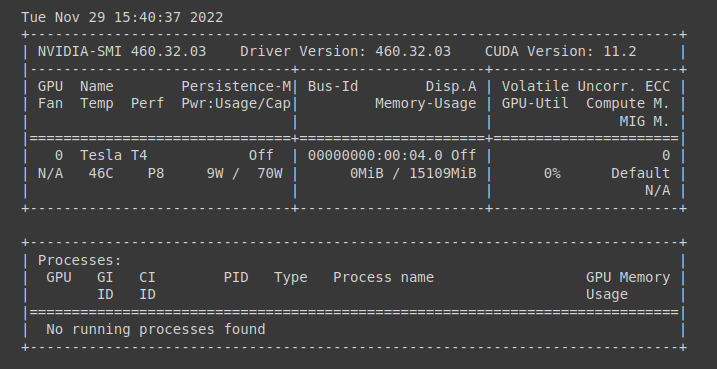
\includegraphics[scale=0.8]{nvidiasmi.png}
\end{center}


\end{document}